%!TEX root = ../thesis.tex
%*******************************************************************************
%****************************** Second Chapter *********************************
%*******************************************************************************

\chapter{Dislocation simulations}

\ifpdf
    \graphicspath{{Chapter2/Figs/Raster/}{Chapter2/Figs/PDF/}{Chapter2/Figs/}}
\else
    \graphicspath{{Chapter2/Figs/Vector/}{Chapter2/Figs/}}
\fi


\section{From molecular dynamics to discrete dislocation dynamics}

In materials science and physics, modeling and simulation play an essential role. In engineering knowledge-based tools are developed to design materials with better performance without unnecessary trials. They are used for quantitative understanding on the relations between composition, processing, structure and properties of the materials. From the materials physics point of view there are great possibilities to test early concepts to describe qualitative findings. Although tremendous potential benefits of modeling and simulation are brought to mankind, they pose challenges because of the huge complexity involving multiple orders of magnitude in time and space scales, mentioning only one of the toughest.
\begin{enumerate}
\item Dislocations bring a clear example of the size scale problems. Dislocation patterning appears on the size scale of hundreds of mean dislocation spacing 
($ \approx $ \SI{10}{\um}), while to resolve dislocation core structure scales below atomic distance are needed
(less than \SI{1}{\angstrom}).
\item Due to the long range interaction the collective motion of dislocation involves rather different different time scales. Creep is a rather slow deformation while the timescale of dislocation motion is short range. This challenge arises e.g.\ at simulating dislocations in single crystal Ni-based superalloys used in aircraft turbine blades: the timescale of dislocation motion is in the order of \si{\us}, while the change in microstructures happens in the order of weeks.
\end{enumerate}
Moreover chemical interactions may play a non-negligible role too. Covering interdisciplinary phenomena whose modelling involves different approaches elevate the problem to a conceptual level. Despite all these difficulties computational models show fruitful promises worth to try. As a general principle the physical accuracy of a model and its practicability are opposite aims regarding the spatial and temporal scales. So minimalist models introducing the smallest possible number of parameters by identifying the essential mechanisms which can capture the phenomenon desired are essential.\footnote{That's why I consider keyboard pushing as science when it comes to simple models based on physical assumptions.}

\subsection{Ab initio}
The starting point of the most fundamental picture in materials' simulation are the wave functions of the nuclei and electrons. ``Schrödinger's equation may solves all\footnote{Richard Feynmann: Lecture on Physics, Volume II, 41–6: Couette flow}'' and describe the time evolution of the system on the level of quantum physics. These models may involve Hartree-Fock and density functional theory approximation, but a key feature is that no phenomenological parameters are introduced. These first principle methods (also known as ab initio) represents the state of the art, completely non-phenomenological methods. First principle methods let us to construct materials have not created yet. It allows to investigate their parameters leading to an improvement in efficiency compared to a completely trial and error experimental discovery of new materials. Due to the complexity of the Schrödinger's equation simulations are strongly limited in both the number of independent variables (particles) and the time length. Their typical values are around \textbf{\numrange{1}{100} atoms} and time range of \textbf{\SIrange{e-15}{e-12}{\second}}. These limitation mean that ab initio methods cannot be used to study the collective properties of dislocations, but the properties of the primitive cell and crystal lattice as the underlying structure for dislocations.

\subsection{Molecular modelling} \label{sec:disloc_sim_md_sim}
Atomic scale methods consider atoms as the smallest units and are essentially build upon the equations of classical mechanics. They do not resolve subatomic scales, i.e.\ nuclei and electrons and their effect taken into account via phenomenological parameters as input parameters of the model leading to the possibility to simulate materials different in structure or in chemical properties. Limitations are moderated compared to ab initio methods: \textbf{\numrange{e4}{e9} or even up to \num{e12} number of atoms} can be handled for up to \textbf{\SIrange{e-12}{e-9}{\second}}. Atomistic methods can be casted into two major categories:
\begin{enumerate}
\item stochastic methods such as Monte Carlo methods\cite{alfonso2015simulation,saito1997monte},
\item deterministic methods such as molecular dynamics (MD\nomenclature[z-MD]{MD}{Molecular dynamics}). MD simulations are capable to simulate dislocation-related properties, such as dislocation-solute atom interaction, interface-matrix dislocation interaction and dislocation-dislocation interaction, creation, and annihilation \cite{ZHANG2013132,doi:10.1080/14786430903081990,Yamakov2002}. Due to computational limitations, they cannot handle large number of dislocations or very slow effects, e.g.\ deformation with a slow strain rate and diffusion controlled processes (like dislocation-climb).
\end{enumerate}

\subsection{Xscopic scale methods}
It is common to distinguish models corresponding to different scales as microscopic, mesoscopic, and macroscopic (denoted by my fantasy name xscopic) scales. They are above atomic scale methods' but their naming is rather arbitrary or field-dependent. Macroscopic scales means the size scale where materials can be handled homogeneous and all phenomena related to atoms can be taken into account via a finite number of parameters and where completely classical approaches can be used. In practice this scale is in the order of \si{\milli\meter} and above. Microscopic scale is directly above atomic scales where ab initio and MD are used. Mesoscale is something in between. In the field of phase/grain microstructures "microscopic" stands for intraphase/intragrain scales and mesoscopic stands for interphase/intergrain scales\cite{Rotersbook}. In fields of dislocation microscopic means that individual dislocations can be resolved (discrete dislocation) and mesoscopic means field quantities (e.g.\ dislocation density or dislocation-dislocation two particle correlation) are introduced to handle dislocated-related phenomena. The work presented in the thesis focuses on dislocations therefore the latter terminology is utilised in the following.

\textbf{Microscopic} methods in this sense mean discrete models like DDD where dislocations resolved into segments along the dislocation line. Forces -- including driving forces, dissipative forces and inertial term -- acting on the whole dislocation is averaged for the segments determining the motion of the segments. Driving force may include various sources, such as external force, dislocation-interaction forces ... etc. DDD simulations provide information on each of the dislocation and they can also handle large number of dislocations even in multiple slip systems to study their evolution during rearrangement. Larger number of dislocations means that with some simplifying assumptions commercially available computers can catch collective dislocation motion phenomena, such as dislocation avalanches \cite{Csikor251,ovaska2015quenched,PhysRevLett.112.235501}. A strong drawbacks of DDD simulations is a trivial outcome of their approach: they resolve dislocations one by one. So since one tries to track the motion of each dislocation segment, the problem leads to computational cost unaffordable at the scales of dislocation patterning.

\textbf{Mesoscopic} methods average out the microstructure: they refers to such models where  fields and continuum quantities are used. As an example, DDD resolved each of the dislocations and tracks their motion, while in CDD modelling dislocation density distributions, dislocation-dislocation correlation functions ... etc. are introduced and their change in time describes the evolution of the system. As a consequent, their computational cost is basically independent of the number of dislocations (or dislocation density) therefore simulation space can be scaled up even to the size scale where real specimen experiments can be performed even on commercial computers. While in DDD models the way stresses are calculated is more or less straightforward, CDD models lead to nontrivial conceptual problems: what are the key quantities, how to handle them mathematically and how could one handle efficiently to a numerical problem. This challenge is not surprising, because CDD models have to link
\begin{itemize}
\item information got from lower-levels contained in discrete models, like the microstate of dislocations and
\item information got from higher-levels describing materials on macroscopic scales.
\end{itemize}
The difficulties mentioned above can be handled by deriving terms and numeric parameters in a continuum models obtained by coherent coarse graining of discrete models. The expected results can be also foreseen by empirically generalise the experimental data in an an adequate way.

\textbf{Macroscopic} scale methods approach the problem from the opposite direction. In this case the evolution of the whole system is prescribed phenomenologically and only finite amount of averaged parameters are used to account for the microstructure. The main advantage of these models is that their numeric implementation is straightforward, they can easily fit into the standard framework of finite element methods already available. These models are efficient engineering tools when it comes to estimate the life-time \cite{Connolly_2014_MST, Le_2014_IJP} under mechanical fatigue or creep conditions. In experiments the details of the stress-strain curves are highly dependent on the specific test conditions hence model parameters must also reflect this sensitivity feature if the underlying constitutive formulation still holds at all. These methods are reliable only in a limited range where they are tested against real experiments meaning their prediction can hardly go beyond what the models were build upon. They are able to capture, however, changing microstructural mechanism by using new set of parameters, i.e.\ introducing new ones and omitting old ones, but this is barely a phenomenological approach where one can hardly give the parameters used in the model any microstructural meaning. Although no doubt that these models provide useful tools in their own field of engineering, they are inadequate for the field of microstructure engineering.


\section{Contiuum dislocation dynamics} \label{sec:disloc_sim_CDD}
The basis of continuum dislocation dynamics was founded by Nye and Kröner in the nineteen fifties by introducing a tensorial measure, the Kröner-Nye dislocation density tensor to represent the geometrically necessary dislocation (GND) \nomenclature[z-GND]{GND}{geometrically necessary dislocation} densities in a crystal. It was cumbersome and took half a decade to describe plasticity with the density field  introduced above in a nontrivial case of continuous dislocation density where one has to already take into account the boundary conditions \cite{doi:10.1080/14786436308213841}. Since then numerous different models based on the Kröner-Nye tensor were introduced \cite{Acharya_2001_JMPS, Le_2016_IJP, Sedlacek_2003_PM, Xia_2015_MSMSE} where dislocations are the boundaries between plastically sheared and unsheared regions on a slip plane. In this picture all dislocations are geometrically necessary and there's no other type of dislocation. In energy functional based models (such as phase field dislocation dynamics model \cite{Beyerlein20150166}) dislocation evolution is driven by the decreasement of the total internal energy, therefore any other source of dislocations than the boundary is neglected. These models can hardly resolve the system spatially below the mean dislocation distance meaning they are inadequate models to account for mechanisms taking place below this size scale.

Another possible type of dislocation is the statistically stored dislocation (SSD) density \nomenclature[z-SSD]{SSD}{statistically stored dislocation} accounted only for the flow stress and plastic slip rate. It neglects completely the geometric compulsion \cite{johnston_1959_JAP, Kocks_1976_JEMT}. These models focus on the reproduction of the connection between dislocation density and the flow stress (e.g.\ the Taylor-equation for the flow stress ${\tau _f} = \alpha GB\sqrt \rho  $, where $G$ is the shear modulus) and the connection between the plastic slip rate (e.g.\ the Orowan-equation $\partial \eta /\partial t = \rho vb$, where $\eta$ is the plastic strain). These descriptions are valid as long as the naive picture of dislocations holds\footnote{tautology} and in these cases they can also describe work hardening and plastic flow \cite{Bouaziz_2013_PM, Caceres_2007_MSEA, Estrin_1984_AM} on a phenomenological base.

In the rest of this work we will focus on another line of approach where individual dislocations are coarse grained only of its own type. These models can account for the evolution of GND and SSD simultaneously \cite{Groma_1997_PRB, Groma_2003_AM}. To minimalise the complexity of such model one could consider only straight edge dislocations in a plain-strain geometry where only two types of dislocations exist: with Burgers vector $s \cdot b$, $s \in \left\{ { +1 , -1 } \right\}$, called 2D dislocation model\footnote{The 3rd direction, $z$, is in the direction of the dislocation line.}. Although the explanation and interpretation of the appearing term in 2D CDD models \cite{Groma_2003_AM} reveals astonishing features \cite{PhysRevB.93.214110}, arbitrary configurations of curved dislocations became examinable with a general extension \cite{Hochrainer_2014_JMPS, hochrainer2007three, Stefan_2011_JMR, SANDFELD20151} granted by a straightforward though cumbersome calculation applied on the original basis. These models have been successfully tested against DDD simulations \cite{Stefan_2015_MSMSE} or against other CDD models \cite{Monavari_2016_JMPS} and proved to be accountable on the size scale below the mean dislocation spacing up to orders of magnitude larger scales.

In the following an above-mentioned 2D CDD model with a statistical approach will be introduced in order to present the basis of chapter \ref{chapter:weakest_link} and \ref{chapter:pattern}.

\subsection{Equation of motion of dislocations}
\nomenclature[z-EOM]{EOM}{equation of motion}
In this section the equation of motion (EOM) of straight, parallel edge dislocations in single slip is discussed from a DDD point of view. This is the simplest setup one can envisage which still reproduces some key features of dislocation system demonstrated by DDD simulations. The derivation is implemented by a systematic manner providing further possibilities for improvement.


\begin{figure}[htbp!] 
\centering    
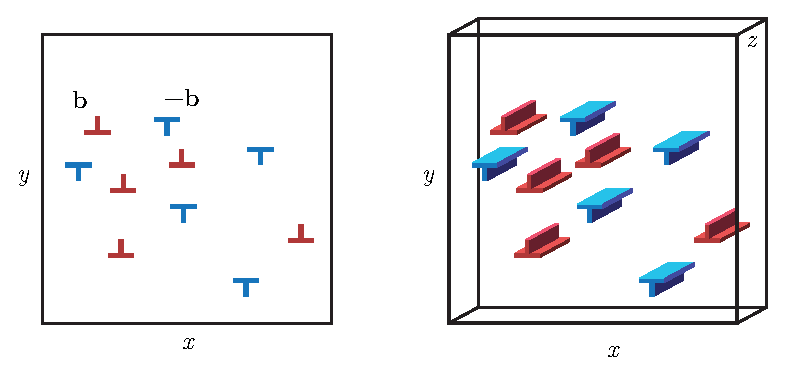
\includegraphics{DDD2}
\caption[2D DDD]{A 2D dislocation configuration (single slip) representing a total of $N = N_t = 10$ dislocations; ${N_ + } = 5$, ${N_ - } = 5$, the number of exceed dislocations ${N_s} = \sum\limits_{i = 1}^N {{s_i}}  = 0$ (s for signed). The $z$ direction is perpendicular to the plane of the sheet/screen and points towards the reader. (The $x$, $y$ and $z$ axes form a right-handed system.)}
\label{fig:2D_DDD}
\end{figure}

In the following we consider $N$ dislocations with Burgers vector $s \cdot \left( {b,0,0} \right)$, $s \in \left\{ { - 1,1} \right\}$ with dislocation line directing to the positive direction of the $z$ axis (see Fig.~\ref{fig:2D_DDD}). Neglecting the inertial terms on dislocations, i.e.\ using over-damped dynamics, the EOM of the dislocation system is given by
\begin{equation} \label{eq:EOM_DDD}
\frac{{d{x_i}}}{{dt}} = {M_0}b{s_i}\left( {\sum\limits_{j = 1}^N {{s_j}{\tau _{{\text{ind}}}}\left( {{{\mathbf{r}}_i} - {{\mathbf{r}}_j}} \right) + {\tau _{{\text{ext}}}}} } \right),
\end{equation}
where ${{\mathbf{r}}_i} = \left( {{x_i},{y_i},{Z_i}} \right)$ is the position ($Z_i$ points to the points of the dislocation line), ${s_i}$ is the sign of the $i$th dislocation, $M_0$ is a mobility factor specific to the dislocation in the system given, $b_i$ is the Burgers vector, ${{\tau _{{\text{ind}}}}}$ is the shear stress generated by dislocation $j$ at the place of dislocation $i$, ${{\tau _{{\text{ext}}}}}$ is the external shear stress. For simplicity the time dependence of ${{\mathbf{r}}_i}$ will not be indicated in the rest of this thesis. The actual form of ${\tau _{{\text{ind}}}}$ reads as
\begin{equation} \label{eq:tau_ind}
{\tau _{{\text{ind}}}}\left( {\mathbf{r}} \right) = x\frac{{{x^2} - {y^2}}}{{{{\left( {{x^2} + {y^2}} \right)}^2}}} = \frac{{\cos \left( \phi  \right)\cos \left( {2\phi } \right)}}{r}.
\end{equation}

By adding a random force term to \cref{eq:EOM_DDD}, the model is capable to contain the effect of thermal noise, leading to a stochastic differential equation. By investigating the corresponding Fokker-Planck equation with real physical parameters, one can find that the time scale corresponding to thermal noises are orders of magnitude (e.g.\ $10^4$) larger then the one corresponding to dislocation-dislocation interaction. Neglecting the thermal fluctuation in the elastic energy resulting that the dislocations cannot escape from even the smallest energy barrier leaving them in the nearest local energy minimum. One has to note that although dislocations are still unstable crystal defects meaning that dislocation-free system would be the preferred configuration, this state cannot be achieved because the system cannot recover from its metastable configuration -- at least within a reasonable time.

Dislocation climb is another thermal effect could have been taken into account. The underlying mechanism lies on vacancies which are stable crystal defects at finite temperature. However, in the followings dislocation climb will be neglected and only glide will be allowed representing a zero-temperature approximation.

\subsubsection{Coarse graining}
The first step towards the desired CDD model from the DDD model is the procedure called coarse graining or homogenisation. The dislocation density tensor introduced by Nye and Kröner is
\begin{equation}
{\alpha _{ij}} =  - {\varepsilon _{ikl}}{\partial _k}\beta _{lj}^{\text{p}},
\end{equation}
where 
$\varepsilon $ is the three-dimensional Levi-Civita symbol\footnote{The completely antisymmetric $3 \times 3 \times 3$ tensor, or the three indexed permutation symbol} and $\beta _{lj}^{\text{p}}$ is the plastic distortion. In the 2D single slip case the quantity ${\alpha _{ij}}$ has only one non-zero component, and it is highly singular on a DDD level: it can be written as a sum of Dirac-delta distributions
\begin{equation} \label{eq:alpha_is_sum_of_dirac_delta}
{\alpha _{31}} = {\rho _{\text{d}}} = \sum\limits_{i = 1}^N {{s_i}\delta \left({{\mathbf{r}} - {{\mathbf{r}}_i}} \right)},
\end{equation}
where ${\rho _{\text{d}}}:{\mathbb{R}^2} \to \mathbb{R}$ denotes the scalar-valued dislocation density. The evolution of the system is completely defined at this point: the EOM of the dislocations are given meaning that the dislocation density can be calculated at any give point at any time which determines -- compared to an initial state -- the plastic distortion and the stress. In this case, however, one has to follow each of the dislocation containing the whole microscopic information of dislocation configuration.

In a hopefully lucky situation one may predict the macroscopic plastic response of the system without knowing the detailed information of the whole dislocation arrangement and the vast majority of the information can be neglected by finding the key homogeneous quantities as it is done in many other physical systems. One way to do that is to calculate locally averaged fields for the dislocation density, dislocation current density, stress, ... etc. Locally averaged means that a convolution is applied with a window function tending to zero fast enough in a certain sense. One may ask if there are only one appropriate function or more, which ones are better and worse and if there exist any window function at all which could provide averaged quantities modelling our system. There is a hope that within certain limits a range of function do the job and the main features of the result obtained by coarse graining does not depend strongly on the specific shape of the window function. If we cannot find any proper function and our model seems to be ineffective describing the reality it may mean that all the microscopic details are necessary for the description and one cannot use a continuum picture.

The goal of the continuum description is to get rid of unimportant details to speed up the numerical models implemented on such basis. However, one has to be careful. Consider two dislocation configurations where signed sum of dislocations are equal within a region, ${N_s} = \sum\limits_{i = 1}^N {{s_i}} $, as seen in Fig.~\ref{fig:coarse_graining}. Apply coarse graining with a window function with the size of box. Consider the signed dislocation density $\kappa$. It can be seen that on one hand the value of $\kappa$ are the same and on the other hand the plastic response of the two configurations are substantially different. This is an example to point out that further quantities than dislocation density tensor is needed to characterise the state of the system.

\begin{figure}[htbp!] 
\centering    
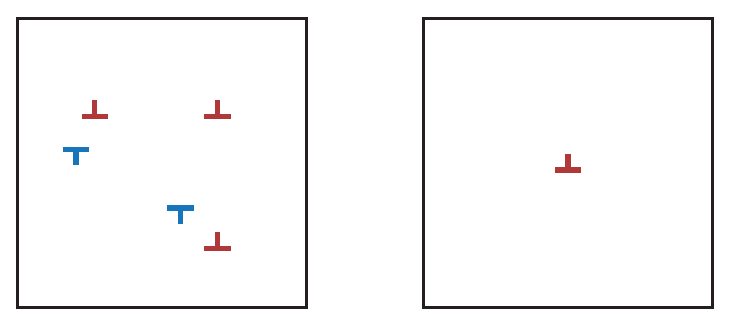
\includegraphics[width=0.8\textwidth]{coarse_graining}
\caption[Coarse graining is riskful]{Coarse graining applied on strongly different dislocation arrangement can lead to the same signed dislocation densities at some points. This two configurations gives the same signed dislocation density $\kappa$ at the center using a window function represented by the box.}
\label{fig:coarse_graining}
\end{figure}


To introduce the key quantities under certain assumptions one has to coarse grain the EOM in \cref{eq:EOM_DDD}. For shorter notation only $s_i=+1$ type of dislocations will be considered first and then the results obtained will be generalised to the case when two types of dislocations are presented. For simplicity, ${\tau _{{\text{ext}}}}$ is neglected first. Let us apply ${\partial _x}\left( {\delta \left( {{\mathbf{r}} - {{\mathbf{r}}_i}} \right) \cdot  \bullet } \right)$ first on both sides:
\begin{equation} \label{eq:EOM_DDD2}
{\partial _x}\left[ {\frac{{d{x_i}}}{{dt}}\delta \left( {{\mathbf{r}} - {{\mathbf{r}}_i}} \right)} \right] = {M_0}{\partial _x}\left\{ {\left[ {\sum\limits_{j \ne i}^N {F\left( {{{\mathbf{r}}_i} - {{\mathbf{r}}_j}} \right)} } \right]\delta \left( {{\mathbf{r}} - {{\mathbf{r}}_i}} \right)} \right\},
\end{equation}
where $F\left( {\mathbf{r}} \right) = b \cdot {\tau _{{\text{ind}}}}\left( {\mathbf{r}} \right)$. With the equivalency
\begin{equation}
{\partial _x}\left( {\frac{{d{x_i}}}{{dt}}\delta \left( {{\mathbf{r}} - {{\mathbf{r}}_i}} \right)} \right) = \frac{{d{x_i}}}{{dt}}{\partial _x}\delta \left( {{\mathbf{r}} - {{\mathbf{r}}_i}} \right) =  - \frac{{d{x_i}}}{{dt}}{\partial _{{x_i}}}\delta \left( {{\mathbf{r}} - {{\mathbf{r}}_i}} \right) =  - \frac{d}{{dt}}\delta \left( {{\mathbf{r}} - {{\mathbf{r}}_i}} \right)
\end{equation}
\cref{eq:EOM_DDD2} reads as
\begin{equation}
 - \frac{d}{{dt}}\delta \left( {{\mathbf{r}} - {{\mathbf{r}}_i}} \right) = {M_0}{\partial _x}\left[ {\left\{ {\int {F\left( {{\mathbf{r}} - {\mathbf{r}}'} \right)} \left[ {{\rho _{\rm{d}}}\left( {{\mathbf{r}}'} \right) - \delta \left( {{\mathbf{r}} - {\mathbf{r}}'} \right)} \right]{d^2}r'} \right\}\underbrace {\delta \left( {{\mathbf{r}} - {{\mathbf{r}}_i}} \right)}_{{\text{avoid self - int}}{\text{.}}}} \right].
\end{equation}
Here the term ${\delta \left( {{\mathbf{r}} - {{\mathbf{r}}_i}} \right)}$ is to avoid self interaction of the dislocations. Recall \cref{eq:alpha_is_sum_of_dirac_delta} and take into account that only positive dislocations are considered and sum up both sides with respect to $i$:
\begin{equation}
 - \frac{d}{{dt}}{\rho _{\rm{d}}}\left( {\mathbf{r}} \right) = {M_0}{\partial _x}\left[ {\left\{ {\int {F\left( {{\mathbf{r}} - {\mathbf{r}}'} \right)} \left[ {{\rho _{\rm{d}}}\left( {{\mathbf{r}}'} \right) - \delta \left( {{\mathbf{r}} - {\mathbf{r}}'} \right)} \right]{d^2}r'} \right\}{\rho _{\rm{d}}}\left( {\mathbf{r}} \right)} \right].
\end{equation}
Please note the non-local property of this equation. Let us make the coarse graining now by applying the operation
\begin{equation}
\left\langle { \bullet \left( {\mathbf{r}} \right)} \right\rangle  = \int { \bullet \left( {{\mathbf{r}}'} \right) \cdot w\left( {{\mathbf{r}} - {\mathbf{r}}'} \right){d^2}r'}  = \left( { \bullet  * w} \right)\left( {\mathbf{r}} \right).
\end{equation}
Denote the averaged one-particle dislocation density function by
\begin{equation} \label{eq:intro_one_particle}
{\rho _1}\left( {\mathbf{r}} \right) = \left\langle {{\rho _{\rm{d}}}\left( {\mathbf{r}} \right)} \right\rangle,
\end{equation}
and the two-particle dislocation density by 
\begin{equation} \label{eq:intro_two_particle}
{\rho _2}\left( {{{\mathbf{r}}_1},{{\mathbf{r}}_2}} \right) = \left\langle {{\rho _{\rm{d}}}\left( {{{\mathbf{r}}_1}} \right){\rho _{\rm{d}}}\left( {{{\mathbf{r}}_2}} \right) - {\rho _{\rm{d}}}\left( {{{\mathbf{r}}_1}} \right)\delta \left( {{{\mathbf{r}}_1} - {{\mathbf{r}}_2}} \right)} \right\rangle.
\end{equation}
With these notation one gets
\begin{equation} \label{eq:one_two_particle_EOM}
\frac{{\partial {\rho _1}\left( {\mathbf{r}} \right)}}{{\partial t}} + M_0 \int {{\partial _x}\left[ {{\rho _2}\left( {{\mathbf{r}},{{\mathbf{r}}_2}} \right)F\left( {{\mathbf{r}} - {{\mathbf{r}}_2}} \right)} \right]{d^2}{r_2} = 0}.
\end{equation}
Please note that in this equation ${\rho _1}\left( {\mathbf{r}} \right)$ and ${\rho _2}\left( {{{\mathbf{r}}_1},{{\mathbf{r}}_2}} \right)$ represent the coarse-grained one- and two-particle densities.

\Cref{eq:one_two_particle_EOM} does not describe completely the system, it contains two time-dependent values ${\rho _1}\left( {\mathbf{r}} \right)$ and ${\rho _2}\left( {{{\mathbf{r}}_1},{{\mathbf{r}}_2}} \right)$. This equation could be used to express the time evolution of the one-particle density function dependent on two-particle density function. However, one can get an equation for the two-particle density function depending on the three-particle density function, ... etc, and in the end the $N-1$-particle density function will depend on the $N$-particle density function. The general equation that gives the dependence of the $k$-particle density function on the $N>k$ particle density function can be found in the work of \citet{Groma_1997_PRB}:
\[\frac{{\partial {f_k}}}{{\partial t}} + \sum\limits_{i = 1}^k {\sum\limits_{j = i,j \ne i}^k {{\partial _{{x_i}}}\left[ {{f_k} \cdot F\left( {{{\mathbf{r}}_i} - {{\mathbf{r}}_j}} \right)} \right]} }  + \left( {N - k} \right)\int {{\partial _{{x_i}}}\left[ {{f_{k + 1}} \cdot F\left( {{{\mathbf{r}}_i} - {{\mathbf{r}}_{k+1}}} \right)} \right]d^2{r_{k + 1}}}  = 0,\]
where the $k$-particle distribution function is introduced, ${\rho _k} = \frac{{N!}}{{k!}}{f_k}$, and it is a function of the coordinates of the dislocations,${f_k}\left( {{{\mathbf{r}}_1},{{\mathbf{r}}_2},...,{{\mathbf{r}}_k}} \right)$, and of the time as well.

With these one got a hierarchy of equations. This form is still equivalent with the description of the original DDD system without the loss of generality, because nothing is supposed on the window function appearing only in the $i$-particle density functions (namely the ${\rho _1}\left( {\mathbf{r}} \right)$ and ${\rho _2}\left( {{{\mathbf{r}}_1},{{\mathbf{r}}_2}} \right)$ in \cref{eq:intro_one_particle,eq:intro_two_particle}). This generality breaks off when one gives a specific function on $w$. In the next two sections different approximation are applied on these terms. It turns out that at least the first  one -- the self-consistent, or mean field -- is an oversimplification while the latter one provides enough to observe dislocation avalanches and dislocation patterning. Before we do so, let us generalise the form of \cref{eq:one_two_particle_EOM} for two different types of dislocations: one with Burgers vector $+b$ and one with $-b$ pointing to the $x$ direction.
\begin{equation} \label{eq:intro_pos_EOM}
\frac{{\partial {\rho _ + }\left( {\mathbf{r}} \right)}}{{\partial t}} =  - {M_0}b{\partial _x}\left\{ {\int {\left\{ {\left[ {{\rho _{ +  + }}\left( {{\mathbf{r}},{{\mathbf{r}}_2}} \right) - {\rho _{ +  - }}\left( {{\mathbf{r}},{{\mathbf{r}}_2}} \right)} \right]{\tau _{{\text{ind}}}}\left( {{\mathbf{r}} - {{\mathbf{r}}_2}} \right)} \right\}{d^2}{r_2}}  + {\rho _ + }\left( {\mathbf{r}} \right){\tau _{{\text{ext}}}}} \right\}
\end{equation}

\begin{equation} \label{eq:intro_neg_EOM}
\frac{{\partial {\rho _ - }\left( {\mathbf{r}} \right)}}{{\partial t}} =  - {M_0}b{\partial _x}\left\{ {\int {\left\{ {\left[ {{\rho _{ -  - }}\left( {{\mathbf{r}},{{\mathbf{r}}_2}} \right) - {\rho _{ -  + }}\left( {{\mathbf{r}},{{\mathbf{r}}_2}} \right)} \right]{\tau _{{\text{ind}}}}\left( {{\mathbf{r}} - {{\mathbf{r}}_2}} \right)} \right\}{d^2}{r_2}}  - {\rho _ - }\left( {\mathbf{r}} \right){\tau _{{\text{ext}}}}} \right\}
\end{equation}

In these equation the two types of ${{\rho _ \pm }}$ and four types of ${{\rho _ {\pm \pm} }}$ represent the coarse grained one- and two-particle density functions.

To get the coarse-grained total dislocation density and signed dislocation density, also known as (coarse-grained) GND, one has to add and then subtract \cref{eq:intro_pos_EOM,eq:intro_neg_EOM}. 
\begin{multline} \label{eq:CDD_rho_wlog}
\frac{{\partial \rho \left( {\mathbf{r}} \right)}}{{\partial t}} =  - {M_0}b{\partial _x}\left\{ \int \left[ {{
   \rho _{ +  + }}\left( {{\mathbf{r}},{{\mathbf{r}}_2}} \right) + {\rho _{ -  - }}\left( {{\mathbf{r}},{{\mathbf{r}}_2}} \right)} \right. \right. \\
  \left. \phantom{\int {\left[ {\left( {\mathbf{r}} \right)} \right]} } {\left.  - {\rho _{ +  - }}\left( {{\mathbf{r}},{{\mathbf{r}}_2}} \right) - {\rho _{ -  + }}\left( {{\mathbf{r}},{{\mathbf{r}}_2}} \right) \right]{\tau _{{\text{ind}}}}\left( {{\mathbf{r}} - {{\mathbf{r}}_2}} \right) d^2r_2}  + \kappa \left( {\mathbf{r}} \right){\tau _{{\text{ext}}}} \right\}
\end{multline}

\begin{multline} \label{eq:CDD_kappa_wlog}
\frac{{\partial \kappa \left( {\mathbf{r}} \right)}}{{\partial t}} =  - {M_0}b{\partial _x}\left\{ \int \left[ {{
  \rho _{ +  + }}\left( {{\mathbf{r}},{{\mathbf{r}}_2}} \right) - {\rho _{ -  - }}\left( {{\mathbf{r}},{{\mathbf{r}}_2}} \right)} \right. \right. \\
  \left. \phantom{\int {\left[ {\left( {\mathbf{r}} \right)} \right]} } {\left.  - {\rho _{ +  - }}\left( {{\mathbf{r}},{{\mathbf{r}}_2}} \right) + {\rho _{ -  + }}\left( {{\mathbf{r}},{{\mathbf{r}}_2}} \right) \right]{\tau _{{\text{ind}}}}\left( {{\mathbf{r}} - {{\mathbf{r}}_2}} \right) d^2r_2}  - \rho \left( {\mathbf{r}} \right){\tau _{{\text{ext}}}} \right\},
\end{multline}
where $\rho  = {\rho _ + } + {\rho _ - }$ and $\kappa  = {\rho _ + } - {\rho _ - }$ are the coarse grained density quantities.

\subsection{Self-consistent field approximation} \label{sec:disloc_sim_self_consistent}
Solving the hierarchy of equations for the different order of dislocation densities is mathematically equivalent with the original problem described in DDD at \cref{eq:EOM_DDD}. The same holds if two types of dislocations are allowed. Instead of introducing higher-rank equations one has to cut them at some rank $k$, i.e.\ to express the $k$-particle density function on lower level particle density functions.

First the simplest possible assumptions will be considered, when the dislocation-dislocation correlation is completely neglected (i.e.\ the hierarchy is cut at $k=2$). In this case according to probability theory the two-particle density function is the direct product of the one-particle density functions:
\begin{equation} \label{eq:no_correlation}
{\rho _{ss'}}\left( {{{\mathbf{r}}_1},{{\mathbf{r}}_2}} \right) = {\rho _s}\left( {{{\mathbf{r}}_1}} \right){\rho _{s'}}\left( {{{\mathbf{r}}_2}} \right)\quad s,s' \in \left\{ { + , - } \right\}.
\end{equation}

By substituting \cref{eq:no_correlation} into \cref{eq:CDD_rho_wlog,eq:CDD_kappa_wlog} one gets
\begin{equation} \label{eq:EOM_no_correlation_rho}
\frac{{d\rho \left( {\mathbf{r}} \right)}}{{dt}} =  - {M_0}b{\partial _x}\left\{ {\kappa \left( {\mathbf{r}} \right)\left[ {{\tau _{{\text{sc}}}}\left( {\mathbf{r}} \right) + {\tau _{{\text{ext}}}}} \right]} \right\}
\end{equation}
and
\begin{equation} \label{eq:EOM_no_correlation_kappa}
\frac{{d\kappa \left( {\mathbf{r}} \right)}}{{dt}} =  - {M_0}b{\partial _x}\left\{ {\rho \left( {\mathbf{r}} \right)\left[ {{\tau _{{\text{sc}}}}\left( {\mathbf{r}} \right) + {\tau _{{\text{ext}}}}} \right]} \right\},
\end{equation}
where
\begin{equation} \label{eq:disloc_int_force}
{\tau _{{\text{sc}}}}\left( {\mathbf{r}} \right) = \left( {\kappa  * {\tau _{{\text{ind}}}}} \right)\left( {\mathbf{r}} \right) = \int {\kappa \left( {{\mathbf{r}}'} \right){\tau _{{\text{ind}}}}\left( {{\mathbf{r}} - {\mathbf{r}}'} \right){d^2}r'}
\end{equation}
is called self-consistent (or mean field) shear stress field, the shear stress generated by the coarse-grained GND. As a side note it is worth to mention calculations can prove that the shear stress introduced here is the same if it were introduced from the field theory of dislocations as the coarse grained quantity of the appropriate component of the stress tensor field $\left\langle {{\sigma _{12}}\left( {\mathbf{r}} \right)} \right\rangle $.

This model also omit the possibility of dislocation creation and annihilation. This could be taken into account to incorporate a model where the dislocation density is not a conservative quantity but in the scope of this thesis this phenomena will be completely neglected. Besides numerical reasons, i.e.\ it requires smaller computational power, a more important reason lies in the nature how such phenomena could be introduced. In 2D systems they always involve new artificial dimensional parameter(s) introducing a new length scale ruining the scale properties of dislocations\cite{0965-0393-22-6-065012}. Natural way to handle dislocation multiplication and annihilation is only given in 3D which is again, out of scope of this thesis.

So we have got the equations for the time evolution of dislocation densities. It should be noted that \cref{eq:EOM_no_correlation_rho,eq:EOM_no_correlation_kappa} could be set up in a completely speculative way too, namely a given dislocation moves in the stress field generated by the other dislocations. The advantage of this method is two-fold. It is pointed out what are the necessary assumptions to obtain it, and this approximation can be improved in a systematic way.

Linear stability analysis shows that within the framework of self-consistent field approximation no perturbation can increase, however, stable perturbation can appear. This means that the elastic interaction between individual dislocations cannot lead to pattern formation which is in agreement with the experiments.

Just to mention a few, the following major issues must be solved.
\begin{itemize}
\item The model does not contain the Taylor-equation for the flow stress ${\tau _f} = \alpha GB\sqrt \rho  $, nor any form of friction-like stress.
\item The elastic energy of a dislocation system where no correlation is introduced diverges logarithmically, an effect not observed experimentally. This would mean that the energy of a dislocation system is not an extensive quantity.
\item No growing perturbation can emerge, the system does not form patterns according to linear stability analysis.
\end{itemize}

\subsection{Dislocation-dislocation correlations} \label{sec:disloc_sim_LDA}
\nomenclature[z-LDA]{LDA}{local density approximation}
To step beyond the self-consistent field approximation one has to consider correlations in the two-particle dislocation density function, which is indeed the case for real systems \cite{PhysRevB.64.224102}. Without loss of generality the two-particle density function can be always written in the form of
\begin{equation}
{\rho _{ss'}}\left( {{{\mathbf{r}}_1},{{\mathbf{r}}_2}} \right) = {\rho _s}\left( {{{\mathbf{r}}_1}} \right){\rho _{s'}}\left( {{{\mathbf{r}}_2}} \right)\left( {1 + {d_{ss'}}\left( {{{\mathbf{r}}_1},{{\mathbf{r}}_2}} \right)} \right)\quad s,s' \in \left\{ { + , - } \right\},
\end{equation}
where ${{d_{ss'}}\left( {{{\mathbf{r}}_1},{{\mathbf{r}}_2}} \right)}$ denotes the so-called dislocation-dislocation correlation function. For a general arrangement of dislocations \cref{eq:one_two_particle_EOM}, the hierarchy of the equations (or in case without restriction on the external stress and the signs of dislocation, \cref{eq:intro_pos_EOM,eq:intro_neg_EOM}) can be used on $d_{ss'}$ to express its form. In case of parallel screw dislocations, one could find an analytical solution if the correlation function can be writtern as a product of two, one-particle function \cite{doi:10.1177/1081286508092609,VINOGRADOV20083726}. In case of edge dislocations, where opposite signs for the Burgers vector is allowed, one has to apply some approximation and find out under what restriction the approximation can be justified.

In the following analysis, a relaxed dislocation system is suspected, where initially each dislocation were placed in an uncorrelated way and the system was allowed to evolve into a state where on each dislocation the acting total stress is zero. (This numeric calculation can be done on DDD modelling.) It is also supposed that the total number of dislocations with opposite Buergers vectors are the same. (Furthermore, no dislocation annihilation or creation is introduced as mentioned before.) The simulation results indicate that the two-particle density functions decay exponentially and due to dimensional reasons, this decay must go with the characteristic length scale of the mean dislocation spacing. Based on this, it assumed that the direct dependency of the two-particle density functions on ${{{\mathbf{r}}_1}}$ and ${{{\mathbf{r}}_2}}$ are weak, and only the difference of the positions of the two particles  occurs in the expressions, the direct dependency of ${{{\mathbf{r}}_1}}$ and ${{{\mathbf{r}}_2}}$ comes only via the spatial dependency of the dislocation density $\rho$, i.e.
\begin{equation}
{d_{ss'}}\left( {{{\mathbf{r}}_1},{{\mathbf{r}}_2}} \right) = {{\tilde d}_{ss'}}\left( {{{\mathbf{r}}_1} - {{\mathbf{r}}_2},\rho \left( {{{\mathbf{r}}_1}} \right)} \right).
\end{equation}
(This approximation is true under the restriction $\kappa  \ll \rho $ \cite{Groma_2003_AM,PhysRevB.93.214110}, and if the dislocation density varies slowly on the length scale of the mean dislocation spacing.) Furthermore the correlation cannot depend on a dimensional argument, therefore supposing the simplest case by dimensional analysis argument one arrives to the form 
\begin{equation} \label{eq:corr_two_particle_dim_arg}
{\tilde d_{ss'}}\left( {{{\mathbf{r}}_1} - {{\mathbf{r}}_2},\rho \left( {{{\mathbf{r}}_1}} \right)} \right) = {\tilde {\tilde {d}}}_{ss'}\left( {\left( {{{\mathbf{r}}_1} - {{\mathbf{r}}_2}} \right) \cdot \sqrt {\rho \left( {{{\mathbf{r}}_1}} \right)} } \right)
\end{equation}
(In the following the tilde is omitted as it does not lead to misreading due to the different number -- or type -- of arguments.) This approximation can be called as local density approximation. This approximation is in perfect analogy with first order approximation applied in conventional thermal systems and leads to linear response theory. By substituting \cref{eq:corr_two_particle_dim_arg} into \cref{eq:CDD_rho_wlog,eq:CDD_kappa_wlog} one gets
\begin{equation}
\frac{{\partial {\rho _ + }\left( {\mathbf{r}} \right)}}{{\partial t}} =  - {M_0}b{\partial _x}\left\{ {{\rho _ + }\left( {\mathbf{r}} \right)\left[ {{\tau _{{\text{sc}}}}\left( {\mathbf{r}} \right) + {\tau _ + }\left( {\mathbf{r}} \right) + {\tau _{{\text{ext}}}}} \right]} \right\}
\end{equation}
and
\begin{equation}
\frac{{\partial {\rho _ - }\left( {\mathbf{r}} \right)}}{{\partial t}} =  + {M_0}b{\partial _x}\left\{ {{\rho _ - }\left( {\mathbf{r}} \right)\left[ {{\tau _{{\text{sc}}}}\left( {\mathbf{r}} \right) + {\tau _ - }\left( {\mathbf{r}} \right) + {\tau _{{\text{ext}}}}} \right]} \right\},
\end{equation}
where ${{\tau _{{\text{sc}}}}\left( {\mathbf{r}} \right)}$ is the previously defined self-consistent stress field and ${{\tau _ + }\left( {\mathbf{r}} \right)}$ and ${{\tau _ - }\left( {\mathbf{r}} \right)}$ are defined as
\begin{equation}
{\tau _ + }\left( {\mathbf{r}} \right) = + \int {\left[ {{\rho _ + }\left( {{\mathbf{r}}'} \right){d_{ +  + }}\left( {{\mathbf{r}} - {\mathbf{r}}'} \right) - {\rho _ - }\left( {{\mathbf{r}}'} \right){d_{ +  - }}\left( {{\mathbf{r}} - {\mathbf{r}}'} \right)} \right]{\tau _{{\text{ind}}}}\left( {{\mathbf{r}} - {\mathbf{r}}'} \right){d^2}r'}
\end{equation}
and
\begin{equation}
{\tau _ - }\left( {\mathbf{r}} \right) =  - \int {\left[ {{\rho _ - }\left( {{\mathbf{r}}'} \right){d_{ -  - }}\left( {{\mathbf{r}} - {\mathbf{r}}'} \right) - {\rho _ - }\left( {{\mathbf{r}}'} \right){d_{ -  + }}\left( {{\mathbf{r}} - {\mathbf{r}}'} \right)} \right]{\tau _{{\text{ind}}}}\left( {{\mathbf{r}} - {\mathbf{r}}'} \right){d^2}r'}.
\end{equation}
Without going into the details, the following observations and assumptions can be made.
\begin{itemize}
\item ${{d_{ +  + }}}$ and ${{d_{ -- }}}$ -- as functions acting on two-particle argument -- are symmetric, therefore the corresponding one-particle variable variants must be even functions of their argument ${\mathbf{r}}$.
\item From a similar argumentation one can get that ${d_{ +  - }}\left( {\mathbf{r}} \right) = {d_{ -  + }}\left( {\mathbf{r}} \right)$ holds.
\item For nearly homogeneous systems the contribution of ${d_{ +  + }} - {d_{ -  - }}$ can be neglected compared to ${d_{ +  - }}$ or ${d_{ -  + }}$.
\item One can apply a Taylor expansion on $\rho \left( {\mathbf{r}} \right)$ and $\kappa \left( {\mathbf{r}} \right)$ around the point ${\mathbf{r}}$.
\item ${\tau _{{\text{ind}}}}\left( {x,y} \right) =  - {\tau _{{\text{ind}}}}\left( { - x,y} \right)$ and ${\tau _{{\text{ind}}}}\left( {x,y} \right) = {\tau _{{\text{ind}}}}\left( { - x, - y} \right)$.
\item ${\tau _{{\text{sc}}}} + {\tau _{{\text{ext}}}}: = {\tau _{{\text{mf}}}}$ is often smaller than other appearing stress quantities (in the case of small GND and low external stress) so on any ${\tau _{{\text{mf}}}}$ depending quantity a Taylor expansion around $0$ can be applied.
\end{itemize}

\subsubsection{Equation of motion in a continuous dislocation dynamic system under local density approximation} \label{sec:EOM_LDA}
The hypotheses mentioned above lead to the equations
\begin{equation} \label{eq:EOM_LDA_rho}
\frac{{\partial {\rho _ + }\left( {\mathbf{r}} \right)}}{{\partial t}} =  - {M_0}b{\partial _x}\left\{ {{\rho _ + }\left( {\mathbf{r}} \right)\left[ {{\tau _{\rm{sc}}}\left( {\mathbf{r}} \right) + {\tau _{\rm{b}}}\left( {\mathbf{r}} \right) - \left( {1 - \frac{{\kappa \left( {\mathbf{r}} \right)}}{{\rho \left( {\mathbf{r}} \right)}}} \right){\tau _{\rm{f}}}\left( {\mathbf{r}} \right) + {\tau _{\rm{d}}} + {\tau _{{\text{ext}}}}} \right]} \right\}
\end{equation}
and
\begin{equation} \label{eq:EOM_LDA_kappa}
\frac{{\partial {\rho _ - }\left( {\mathbf{r}} \right)}}{{\partial t}} =  + {M_0}b{\partial _x}\left\{ {{\rho _ - }\left( {\mathbf{r}} \right)\left[ {{\tau _{\rm{sc}}}\left( {\mathbf{r}} \right) + {\tau _{\rm{b}}}\left( {\mathbf{r}} \right) - \left( {1 + \frac{{\kappa \left( {\mathbf{r}} \right)}}{{\rho \left( {\mathbf{r}} \right)}}} \right){\tau _{\rm{f}}}\left( {\mathbf{r}} \right) - {\tau _{\rm{d}}} + {\tau _{{\text{ext}}}}} \right]} \right\},
\end{equation}
or equivalently by adding and subtracting them:
\begin{equation}
\frac{{\partial \rho \left( {\mathbf{r}} \right)}}{{\partial t}} =  - {M_0}b{\partial _x}\left\{ {\kappa \left( {\mathbf{r}} \right)\left[ {{\tau _{{\rm{sc}}}}\left( {\mathbf{r}} \right) + {\tau _{\rm{b}}}\left( {\mathbf{r}} \right) + {\tau _{{\text{ext}}}}} \right] + \rho \left( {\mathbf{r}} \right){\tau _{\rm{d}}}\left( {\mathbf{r}} \right)} \right\}
\end{equation}
and
\begin{equation} \label{eq:pattern_eom_kappa}
\frac{{\partial \kappa \left( {\mathbf{r}} \right)}}{{\partial t}} =  - {M_0}b{\partial _x}\left\{ {\rho \left( {\mathbf{r}} \right)\left[ {{\tau _{{\rm{sc}}}}\left( {\mathbf{r}} \right) + {\tau _{\rm{b}}}\left( {\mathbf{r}} \right) + \frac{{{\kappa ^2}\left( {\mathbf{r}} \right) - {\rho ^2}\left( {\mathbf{r}} \right)}}{{{\rho ^2}\left( {\mathbf{r}} \right)}}{\tau _{\rm{f}}}\left( {\mathbf{r}} \right) + {\tau _{{\text{ext}}}}} \right] + \kappa \left( {\mathbf{r}} \right){\tau _{\rm{d}}}\left( {\mathbf{r}} \right)} \right\},
\end{equation}
where the leading terms ${{\tau _{\rm{b}}}\left( {\mathbf{r}} \right)}$, ${{\tau _{\rm{d}}}\left( {\mathbf{r}} \right)}$ and ${{\tau _{\rm{f}}}\left( {\mathbf{r}} \right)}$ reads as 

\begin{equation} \label{eq:flow_stress}
{\tau _{\rm{f}}}\left( {\mathbf{r}} \right) =  - \mu bC\sqrt {\rho \left( {\mathbf{r}} \right)},
\end{equation}
\begin{equation}\label{eq:back_stress}
{\tau _{\rm{b}}}\left( {\mathbf{r}} \right) =  - Gb\frac{D}{{\rho \left( {\mathbf{r}} \right)}}{\partial _x}\kappa \left( {\mathbf{r}} \right),
\end{equation}
and 
\begin{equation}\label{eq:diff_stress}
{\tau _{\rm{d}}}\left( {\mathbf{r}} \right) =  - Gb\frac{A}{\rho \left( {\mathbf{r}} \right) }{\partial _x}\rho \left( {\mathbf{r}} \right),
\end{equation}
where $\mu$ is the shear modulus, $\nu$ is the Poisson's ratio and $G = \mu /\left[ {2\pi \left( {1 - \nu } \right)} \right]$. $C$, $D$ and $A$ are parameters in the order of $1$, they depend on some of the one- and two-particle density functions, but while $A$ and $D$ are constants under the assumptions mentioned above, $C$ is linear in ${\tau _{{\text{mf}}}}$. Let us take a close look on the parameters and the stress terms.
\begin{enumerate}
\item To have a more precise description on $C$, the strain rate from dislocation field theory must be included at this point. Without further explanation we recall \cite{gromaCISM} that the plastic shear rate for a homogeneous system can be expressed as 
\begin{equation}
\dot \gamma  = \rho b{M_0}\left[ {{\tau _{{\text{mf}}}} - \left( {1 - \frac{{\kappa {{\left( {\mathbf{r}} \right)}^2}}}{{\rho {{\left( {\mathbf{r}} \right)}^2}}}} \right){\tau _{\rm{f}}}\left( {\mathbf{r}} \right)} \right].
\end{equation}
For a system where $\kappa = 0$ the flow stress will have a finite value due to dislocation dipoles and multipoles, and below this shear stress value the plastic strain rate is 0. The relation
\begin{equation} \label{eq:friction_stress_coeff}
C = \left\{
  \begin{array}{lr}
    \frac{\alpha }{\mu b \sqrt \rho  } \tau_{\text{mf}} & {\text{if }}{\tau _{{\text{mf}}}} \leqslant {\tau _{\text{flow}}} \\ 
  \alpha \quad  & {\text{otherwise,}}
  \end{array}
\right.
\end{equation}
does reflect this behavior, where ${\tau _{{\text{flow}}}} = \alpha \mu b\sqrt \rho  $ is the flow-stress. One can envisage then the role of the mean-field stress as the driving force in a stick-slip-like system making it a good argument to call ${{\tau _{\rm{f}}}}$ as friction stress. $\alpha$ is a parameter in the model depending on the microstructure of the dislocation arrangement.

It is nontrivial how a case-separated value like \cref{eq:friction_stress_coeff} can be obtained from an energy functional if one tries to construct this dependency by a variational approach. The key idea is to add a nontrivial, nonlinear mobility function with a threshold by hand. These terms play the role of Taylor stresses, i.e.\ they represent the positive and negative dislocations trapping each other into a $n$-polar configuration. Please note the role of $\kappa$ in \cref{eq:EOM_LDA_kappa,eq:EOM_LDA_rho}, as in the case of excess dislocations of type ${\rho ^i},\;i \in \left\{ { + , - } \right\}$ the pinning force is reduced for $\rho^i$ and increased for the other type. As a special case, $\kappa  = \rho $ or $\kappa  = -\rho $, the pinning stress is $0$.
\item 
To name the term $\tau_{\rm{b}}$ note the relation ${\tau _{\rm{b}}} \sim {\partial _x}\kappa $. Such term is often used in strain gradient plasticity theories accounting for size effects. It is called the term back stress, therefore this term will be referred as back stress. A main difference here is that it is introduced with no further physical parameters then the already used ones and the appearing length scale appears through the (mean) dislocation spacing $\sqrt{\rho}$.
\item
The term $\tau_d$ is called diffusion stress because it goes with the derivative of the dislocation density $\rho$, ${\tau _d} \sim {\partial _x}\rho $. It's atypical feature is that it moves both positive and negative dislocations the same direction, as can be seen on \cref{eq:EOM_LDA_rho,eq:EOM_LDA_kappa}.
\end{enumerate}

These results are valid under many limitations, e.g.\ $\kappa  \ll \rho $, but the model can be extended by a phase-field approach to cases when $\kappa  \approx \rho $ \cite{PhysRevLett.114.015503}. For general $\kappa / \rho$ cases there is no reason not to use linear interpolation between the two extremities. Further extensions towards a 3D description is also possible \cite{PhysRevB.92.174120}. 

\subsection*{Summary}
It was explicated why and how one can to move further than DDD-level description in order to handle samples in the size scales of microns. It has to be realised, that continuum description raises conceptional and mathematical difficulties. They can be solved by either ad-hoc empirical approaches suitable for complex systems using fitting parameters which meanings are hardly possible to express on a microstructural level or analysing the simplest cases which can be handled as exact as possible with parameters which meanings are clear on a microstructural level. The latter way was followed and elaborated in a CDD model based on the simplest case of DDD, a single slip system with straight edge dislocations. It was pointed out what approximations lead to non-physical results, e.g.\ considering no correlation between dislocations and it is showed what minimal further step could be added to achieve a description which shows no inconsistency\footnote{up to date today}.

This simplest case used above represents real setups with real specimen meaning that this description is valid not only a set with measure zero. This description is exact in the sense that the meaning of all quantities introduced are well understood and direct derivation can be set up from a corresponding DDD model.

We may want, however, to introduce further simplification in order to solve the EOM of the given quantities of $\kappa$ and $\rho$, or equivalently, $\rho_+$ and $\rho_-$. The robustness of the calculation is demonstrated in chapter \ref{chapter:weakest_link} where further assumptions will be considered to achieve an even more minimal picture of dislocation rearrangement. Although the derivation explained above require strong simplifications, the advantage of this approach, namely that the final model is got by dropping out terms and take stronger and stronger assumptions, is that it remains clear, what are the assumptions required, in contrast to a merely ad-hoc approaches where the validity is completely non-controlled.

The model derivated requires -- beside the material-specific Poissons ratio and shear modulus -- three parameters depending on the dislocation-arrangement, namely $A$, $D$ and $C$. The first two can be considered constant but for $C$ one may consider a more accurate value as it can be accounted for the stochastic behaviour of dislocation systems. A step back from CDD towards DDD could be made in order to figure out how to bestow $C$ to represent the microstructural property leading to stochastic behaviour during dislocation avalanches. In chapter \ref{chapter:weakest_link} besides further simplification an assumption will be made which is not linked directly to this pioneering derivation of CDD.
